\documentclass[a4paper,11pt]{article}
\usepackage{ml}
\usepackage{mlsubmit}
\usepackage{url}
\usepackage{graphicx}
\graphicspath{ {./} }
\newcommand\tab[1][1cm]{\hspace*{#1}}\begin{document}

\initmlsubmision{1} % assignment number
{Lt Cdr Rahul Raj}   % your name
{18111053}	% your roll number

\begin{mlsolution}
\section*{Sub Question (1)  Misclassification Rate	}

\tab Classification Error is one of the methods to measure the purity or homogenity of set of datapoints. It is calculated as below, \footnote{https://www-users.cs.umn.edu/~kumar001/dmbook/ch4.pdf}
$$Err(Node) = 1 - \max\limits_{i} [P(i|Node] $$ 
\begin{center}

\tab where $i\ \epsilon\ \{1,0\}$\\
\end{center}
\tab Therefore, Misclassification rate is calculated as\footnote{https://sebastianraschka.com/faq/docs/decisiontree-error-vs-entropy.html}
\begin{align*} 
  \textbf{Misclassification Rate} &= Err_{Before\ split} - Err_{After\ split}
\end{align*}
\begin{align*}
\text{where\ }
Err_{After\ split} &= \sum\limits_{i\ \epsilon\ child node} {P(i) \times Err(i)}
\end{align*}
\noindent
\tab Therefore, classification error of dataset as per given setting is as follows
\begin{align*} 
  Err_{Before\ split} &= 1 - \max(P({0}),P({1}))\\
  &= 1 - \max(P(400),P(400))\\
  &= 1 - \frac{1}{2}\\
  &= 0.5
\end{align*}

\noindent
\tab Calculating the Error for  Left Node and Right Node of Tree A\\
\begin{equation*}
  \begin{split}
    Err(A_{Left}) &= 1 - \max\ [P(A_{Left})]\\
    &= 1 - \max\ (P(0), P(1))\\
    &= 1 - \frac{3}{4}\\
    &= 0.25
  \end{split}
\quad\linebreak\quad
  \begin{split}
    Err(A_{Right}) &= 1 - \max\ [P(A_{Right})]\\
    &= 1 - \max\ (P(0), P(1))\\
    &= 1 - \frac{3}{4}\\
    &= 0.25
  \end{split}
\end{equation*}

\noindent
\begin{align*}
\text{Therefore\ } Err_{After\ split} &= \frac{400}{800} \times 0.25 + \frac{400}{800} \times 0.25\\
 &= 0.25
\end{align*}
\tab \textbf{Misclassification Rate of Tree A} $= Err_{Before\ split} - Err_{After\ split}$
\begin{align*}
  &=(0.5) - (0.25)\\   
  &= \textbf{0.25}\ or\ \textbf{25\%}
\end{align*}
\noindent
\tab The mislassification rate of \textbf{Tree B} is also calculated in same way\\
\\
\tab \textbf{Misclassification Rate of Tree B}$= Err_{Before\ split} - Err_{After\ split}$
\begin{align*}
  &=(0.5) - (0.25)\\   
  &= \textbf{0.25}\ or\ \textbf{25\%}
\end{align*}
\subsection*{Observations}
\tab From the above calculations, it is observed that the misclassificaiton rates of both TreeA and Tree B are same i.e 25\%. 
\subsection*{Conclusion}
\tab If misclassification rate is considered as measure of purity, growing the decision tree further through Tree A or TreeB will not yeild a better fit for the model. 

\section*{Sub Question (2)  Information Gain	}
\tab Entropy is another way to measure the purity or homogenity of set of datapoints. High Entropy means less purity. Entropy is calculated as follows,
$$H(S)\ =\ -\sum\limits_{c\  \epsilon\  C} {P_c \times Log_2 P_c}$$
\noindent
\tab \tab \tab \tab where $P_c$ is the probability of Class C\\\\
\noindent
\tab \textbf{Information Gain is the difference between Entropy before and after splitting dataset.}
Entropy of dataset before split is calculated as follows,
\begin{align*} 
  H(S_{Before\ split}) &= \ -\sum\limits_{c\  \epsilon\  C} {P_c \times Log_2 P_c}\\
  &= -\ (P(0) \times\ Log_2\ P(0)\ +\ P(1) \times\ Log_2\ P(1))\\
  &= -\ (\frac{1}{2} \times Log\ \frac{1}{2} + \frac{1}{2} \times Log\ \frac{1}{2} )\\
  &= 1
\end{align*}

\noindent
\tab Calculating the Entropy for  Left Node and Right Node of Tree A\\
\begin{equation*}
  \begin{split}
    H(A_{Left}) &=  -\ (\frac{3}{4} \times Log\ \frac{3}{4} + \frac{1}{4} \times Log\ \frac{1}{4} )\\
    &= 0.81125
  \end{split}
\quad\linebreak\quad
  \begin{split}
    H(A_{Right}) &=  -\ (\frac{1}{4} \times Log\ \frac{1}{4} + \frac{3}{4} \times Log\ \frac{3}{4} )\\
    &= 0.81125
  \end{split}
\end{equation*}
\begin{align*}
\text{Therefore,\ }H(S_{After\ split}) &= \sum\limits_{c\  \epsilon\  C}  \frac{|H(s_c)|}{|H(s)|}) {\times H(S_c)}\\
 &= (\frac{400}{800} \times 0.81125) + (\frac{400}{800} \times 0.81125) \\&=\ 0.81125
\end{align*}
\tab The Information Gain (IG$_A$) of \textbf{Tree A} calculated as\\
\\
\tab \textbf{Information Gain (IG$_A$)} $= H(S_{Before\ split})\ -H(S_{After\ split})$
\begin{align*}
  &=1-(0.81125)\\
  &= \textbf{0.18875}
\end{align*}
\noindent
\tab Similarly, Information Gain (IG$_B$) of \textbf{Tree B} is calculated as\\
\\
\tab \textbf{Information Gain (IG$_B$)} $= H(S_{Before\ split})\ -H(S_{After\ split})$
\begin{align*}
  &=1-((\frac{600}{800} \times 0.917628) + (\frac{200}{800} \times 0))\\   
  &=1-(0.68872)\\   
  &= \textbf{0.31128}
\end{align*}
\subsection*{Observations}
\tab From the above calculations, it is seen that the IG of Tree B is higher than the IG of Tree A.  Information Gain is an indicator on change in purity of dataset while undertaking split at that point. 
\subsection*{Conclusion}
\tab Since IG$_B$ \textgreater\ IG$_A$, we will prefer Tree B for further growing the Decision Tree.
\section*{Sub Question (3) Different Answers for Sub Questions (1) and (2)}
\subsection*{Observations}
\tab From the above, it is seen that the misclassification rate is same for Tree A and Tree B. This implies that the classification error reduces uniformly by choosing either Tree A or Tree B. Therefore, decision tree is complete in this case.
\noindent\\
\\
\tab However, when we choose Entropy as measure of purity, we observed that the Information Gain (IG) is higher when we choose Tree B. This means Tree B is preferred for further growing the decision Tree.
\subsection*{Conclusion}
\tab Decision Tree can be grown further if the Entropy is preferred over misclassification rate as measure of purity of the dataset.

\

\end{mlsolution}

\begin{mlsolution} 
\section*{Consistency of 1-NN Classifier}
\tab Benchmark for analyzing the performance of Nearest Neighbor classifier is the \textbf{Bayes Error Rate}, denoted by $R^*$. As rule of thumb, no classifier can have error rate less than $R^*$. Upper and lower bound of $R^*$ is as follows \footnote{Book by Gilbert Harman and Sanjeev Kulkarni, \textit{An Elementary Introduction to Statistical Learning Theory}} \\
$$ 0 \quad \leq \quad R^* \quad \leq \quad \frac{1}{2} $$
\noindent
\tab Let $R_n$ denotes the expected error rate after n training examples. We are interested in the consistency of the 1-NN classifier while number of training examples tends to infinity $i.e\ n \rightarrow \infty$ denoted by $R_\infty $. Lower bound of $R_\infty $ is $R^*$. Upper bound in terms of $R^*$ is $2R^* \left( 1 - R^* \right)$ \footnote{Proof at Para 4.5.3 in Book by Duda and Hart, \textit{Pattern Classification}}. This is equivalent to $2 \times R^*$, since error rate must be between 0 and 1.Therefore, 
$$ 0 \quad \leq \quad R_\infty \quad \leq \quad 2 \times R^* $$
\noindent
\tab This means in worst case also, the NN classifier will not have error rate more than twice the Bayes Error Rate, provided the number of training examples tend to infinity. Intuitively, as the number of training data increases, the distance between test example and its nearest neighbor tends to zero. While computing $R_\infty$, it is as though the distance is zero. 
\subsection*{Noise Free setting}
\tab In a noise free setting where every training example is labeled correctly, the Bayes Error Rate is zero. $i.e. R^* = 0 $. Therefore, as per the upper bound described above, $R_\infty$ will also be zero. 
\subsection*{Conclusion}
\noindent
\tab It is concluded that the 1-NN classifier is consistent and approaches Bayes Optimal Error Rate, when number of training examples tends to infinity. Assuming that the data is independently and identically distributed over feature space and Euclidean norm is used for establishing the Nearest Neighbor, Stone\footnote{Stone, C.,
\textit{Consistent Nonparametric Regression}, Annals of Statistics, 1977.} has already proved that the NN classifier is universally consistent.

\end{mlsolution}

\begin{mlsolution}

\section*{Linear Regression meets Nearest Neighbors}
\tab For unregularized Linear Regression the model, closed form solution is $\hat{w} = (X^TX)^{-1}X^Ty$
\begin{center}
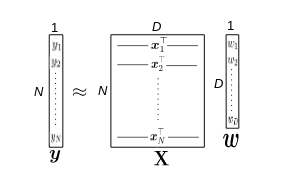
\includegraphics[scale=.5]{linreg}

\end{center}
\noindent
\tab Prediction of a new test input $x_*$ is expressed as \noindent 
\begin{align*}
  y_* &= f(x_*)\\
  &= {w_n}^Tx_*\\
  &= {x_*}^Tw_n\\
  &= {x_*}^T(X^TX)^{-1}X^Ty
\end{align*}

\noindent
\tab Here we can observe that the expression for $w_n$ is ${x_*}^T(X^TX)^{-1}X^T$.
\subsection*{Conclusion}
\tab When ever a new input $x_*$ is given, the corresponding weight $w$ is calculated as the inner product of $x_*$ with $(X^TX)^{-1}X^T$. Therefore, the calculation of the weight $w$ in case of linear regression depends on the dimension $D$ of the test input. (As seen in the above figure)\\

\noindent
\tab However, in the case of weighted K - Nearest Neighbor Algorithm, the weight $w_n$ is the inverse distance of 'K' nearest neighbors only. It does not assume any explicit function $f(x_*)$. Moreover, for calculating distance, any metric such as Euclidean, Manhatton, etc. can be used. In a weighted KNN algorithm, weight is applied to all the training data points and thus causing algorithm to run slower. \footnote{http://www.data-machine.com/nmtutorial/distanceweightedknnalgorithm.htm }

\end{mlsolution}

\begin{mlsolution}

\section*{Feature specific $l_2$ regularization}
\noindent
\tab Regularized least squares regression objective function is written as
$$
\sum\limits_{n=1}^{N}(y_n-w^Tx_n)^2 + \frac{\lambda}{2}w^Tw
$$
\noindent
\tab Alternate solution by applying regularizer to each of the $w_d$ can be derived as follows\\
\noindent
\tab 
\begin{align*}
arg\ min\ (Y-XW)^T(Y-XW) + \frac{\lambda}{2}W^TW\\
(Y-XW)^T(Y-XW) + W^T \lambda W \\
\textnormal{Where, $\lambda$ be a matrix of regularizers of size $D \times D$.}\\
\textnormal{Taking derivative and equating to zero to get closed form solution}\\
\frac{d }{dW}(Y-XW)^T(Y-XW) + W^T \lambda W &= 0\\
\frac{d }{dW}(Y^T-W^TX^T)(Y-XW) + W^T \lambda W &= 0\\
\frac{d }{dW}(Y^TY-W^TX^TY-Y^TXW+W^TX^TXW) + W^T \lambda W &= 0\\
\frac{d }{dW}(Y^TY-2W^TX^TY+W^TX^TXW) + W^T \lambda W &= 0\\
\frac{d }{dW}(Y^TY) - \frac{d }{dW}(-2W^TX^TY)+\frac{d }{dW}(W^TX^TXW) + \frac{d }{dW}(W^T \lambda W) &= 0\\
0 - 2X^TY + 2X^TXW + \lambda W +\lambda ^T W&= 0\\
\textnormal{Since Matrix $\lambda$ is assumed to a diagonal matrix. $\lambda = \lambda^T$. Therefore,}\\
0 - 2X^TY + 2X^TXW + 2\lambda W &= 0\\
(X^TX + \lambda) W &= X^TY\\
 W &= (X^TX + \lambda)^{-1}X^TY\\
\end{align*}
\subsection*{Conclusion}
\tab Closed form solution of weight vector 
$$
w = (X^TX + \lambda)^{-1}X^TY
$$
\end{mlsolution}
	
\begin{mlsolution}
\section*{Multi-output Regression with Reduced Number of Parameters}
\noindent \tab Problem reduces to 
$$
\hat{S} = arg\ min\ TRACE[(Y-XBS)^T(Y-XBS)]
$$
\begin{align*}
\textnormal{Taking derivative and equating to zero to get closed form solution}\\
\frac{d }{dS}TR[(Y-XBS)^T(Y-XBS)] &= 0\\
\frac{d }{dS}TR[(Y^T-S^TB^TX^T)(Y-XBS)]&= 0\\
\frac{d }{dS}TR[(Y^TY-S^TB^TX^TY-Y^TXBS+S^TB^TX^TXBS)]&= 0\\
\frac{d }{dS}TR[(Y^TY-2S^TB^TX^TY+S^TB^TX^TXBS)]&= 0\\
0-2B^TX^TY+B^TX^TXBS +(B^TX^TXB)^TS)&= 0\\
(B^TX^TXB)S&= B^TX^TY\\
S&= (B^TX^TXB)^{-1}B^TX^TY\\
\end{align*}
\subsection*{Observation}
\noindent \tab It is observed that the closed form solution is $S = (B^TX^TXB)^{-1}B^TX^TY$ and similar to expression $S = (Z^TZ)^{-1}Z^TY$ where $Z=XB$. In other words, $Z$ is a transformed version of $X$. Here  $X$ is of dimension $N \times D$ and $B$ is of dimension $D\times K$. Therefore, $Z$ will be of dimension $N \times K$. This means that the number of columns of $X$ has been reduced from $N$ to $K$. This is actually a reduction in parameters/ dimensions in $X$.
\subsection*{Conclusion}
\noindent \tab  Entire exercise of converting $W$ to $B\times S$ can be viewed as a step for dimensionality reduction and the factor affecting the same is the value chosen for $K$.
\end{mlsolution}

\begin{mlsolution}

\section*{Test Set Classification Accuracy - Method 1}

\tab Refer to attached "convex.py" file for implementation in Python. Details of Test-set predictions from implemented model is as tabulated below

\begin{center}
    \label{tab:table1}
    \begin{tabular}{l|c|r} % <-- Alignments: 1st column left, 2nd middle and 3rd right, with vertical lines in between
      \textbf{Ser} & \textbf{Total correct predictions} & \textbf{Accuracy}\\
      \hline
      (a) & 2898 out of 6180 & 46.8932 \%
    \end{tabular}
\end{center}

\section*{Test Set Classification Accuracy - Method 2}
\noindent
\tab Refer to attached "regress.py" file for implementation in Python. Details of Test-set predictions from implemented model is as tabulated below

\begin{center}
    \label{tab:table1}
    \begin{tabular}{l|c|c|l} % <-- Alignments: 1st column left, 2nd middle and 3rd right, with vertical lines in between
      \textbf{Ser} & \textbf{Total correct predictions} & \textbf{Accuracy} & \textbf{lambda($\lambda$)}\\
      \hline
      (a) & 3590 out of 6180 & 58.0906 \% & 0.01\\
      (b) & 3680 out of 6180 & 59.5469 \% & 0.1\\
      (c) & 4165 out of 6180 & 67.3948 \% & 1\\
      (d) & 4529 out of 6180 & \textbf{73.2848 \%}  &\textbf{10} \color{red} $\leftarrow$ \text{Highest accuracy} \\
      (e) & 4430 out of 6180 & 71.6828 \% & 20\\
      (f) & 4022 out of 6180 & 65.0809 \% & 50\\
      (g) & 3490 out of 6180 & 56.4725 \% & 100\\
    \end{tabular}
\end{center}
\subsection*{Instructions for running the program } 

\tab Python version 3.5 has been used for implementation of above methods \footnote{ with help of official documentations and online resources}\\
\\
\noindent
\tab For Method 1\\
\tab \tab Step 1. Copy the "convex.py" file to the folder containing the data \\
\tab \tab Step 2. Execute the program from terminal\\
\\
\tab For Method 2\\
\tab \tab Step 1. Copy the "regress.py" file to the folder containing the data\\
\tab \tab Step 2. Execute the program from terminal\\
\\


\end{mlsolution}


\end{document}
